\section{Cache com Ruby on Rails}

Em aplicações web, especialmente no contexto do \textit{Rails}, o conceito de \textit{cache} refere-se à prática de armazenar conteúdos gerados durante o processamento de requisições para posterior utilização em requisições subsequentes. O \textit{Ruby on Rails} fornece em sua API uma interface única e genérica que possibilita maneiras de integrar-se com sistemas terceiros que atuam como bases de dados para armazenamento de \textit{cache}. Isso oferece ao programador a flexibilidade de escolher estratégias de como um dado específico será armazenado, tornando também a tarefa de definir a expiração dos dados armazenados mais simples, algo que, quando feito manualmente, é bastante suscetível a erros. Na seção \ref{sec:tipos_de_cache_no_ruby_on_rails} é explorada as maneiras que o \textit{Rails} permite com que o programador utilize sua interface de \textit{cache}, e na seção \ref{sec:bases_de_dados_para_cache_no_ruby_on_rails} são explicadas as principais interfaces disponibilizadas pelo \textit{Rails} para comunicação com bases de dados para \textit{cache} \cite{caching-with-rails-overview}.

\subsection{Tipos de cache no Ruby on Rails}
\label{sec:tipos_de_cache_no_ruby_on_rails}

O \textit{Ruby on Rails} fornece maneiras de se utilizar \textit{cache} com funcionalidades embutidas, ou com \textit{gems} que se integram com o \textit{framework} sem muita dificuldade. A seguir são descritas cada uma dessas maneiras com suas particularidades, pontos positivos e negativos.

\subsubsection{Page Caching}

O \textit{page caching} é uma estratégia de \textit{cache} fornecida pela \textit{gem}  \textit{actionpack-page\_caching}, que consiste em salvar o conteúdo de uma requisição em um arquivo estático que será servido como resultado nas próximas requisições. Dessa maneira, uma vez salvo o resultado de uma requisição específica, quando realizada uma nova requisição ao mesmo \textit{endpoint}, o arquivo salvo será servido pelo servidor, de tal forma que a requisição sequer será processada pela aplicação \textit{Rails}. Essa abordagem apesar de simples, possui potencial para reduzir bastante o \textit{response time} da aplicação para os \textit{endpoints} que forem armazenados.

Porém, esta estratégia funciona apenas para requisições \textit{get} e \textit{head} com retorno de código 200. A utilização desse mecanismo de \textit{cache} também não é recomendada para páginas que requiram autenticação, pois a aplicação \textit{Rails} precisa decidir se o remetente da requisição está ou não autorizado a receber o conteúdo solicitado \cite{actionpack-page-caching}.

A \textit{gem actionpack-page\_caching} está disponível em seu repositório oficial no endereço \href{https://github.com/rails/actionpack-page_caching}{https://github.com/rails/actionpack-page\_caching}.

\subsubsection{Action Caching}

O \textit{action caching} é similar ao \textit{page caching} no sentido de que a resposta inteira será armazenada. Essa estratégia de \textit{cache} é fornecida pela \textit{gem actionpack-action\_caching}. Entretanto, nessa abordagem a requisição passa a ser recebida pela aplicação \textit{Rails}, ao ponto que os filtros são executados antes do \textit{cache} ser servido. Isto é, caso o \textit{endpoint} consultado requira autenticação para decidir se um determinado recurso será ou não servido, por exemplo, as verificações serão realizadas na \textit{controller}, para só então o conteúdo em \textit{cache} ser servido.

O \textit{action caching} permite que o programador especifique diretamente o tempo de vida de um armazenamento de \textit{cache} a nível de \textit{actions} dentro da \textit{controller}, além de permitir especificar condições para decidir se o resultado de uma \textit{action} será ou não servido por \textit{cache} \cite{actionpack-action-caching}.

\subsubsection{Fragment Caching}

Aumentando ainda mais o nível de granularidade do armazenamento de informação em \textit{cache}, o \textit{Rails} fornece um mecanismo chamado \textit{fragment caching}. Com o \textit{fragment caching} é possível armazenar fragmentos específicos do \textit{template} de uma \textit{view}, ao invés de armazena-la por inteira. Essa abordagem é especialmente utilizada em trechos da \textit{view} onde objetos de \textit{models} são renderizados.

Quando o \textit{Rails} se depara com um fragmento de \textit{view} que exibirá informações de um objeto de uma \textit{model}, e que há a instrução de armazenar o resultado em \textit{cache}, uma chave única será criada com base na junção do nome da \textit{view}, o nome da \textit{model} do objeto em questão, o \textit{id} e o atributo \textit{updated\_at} do objeto, que representam a chave primária e o momento em que o objeto foi atualizado pela última vez, respectivamente. Caso não exista um valor já armazenado em \textit{cache} para esta chave, o fragmento será renderizado pela aplicação e o resultado será armazenado na memória com associação direta à essa chave \cite{caching-with-rails-overview}.

\subsubsection{Russian Doll Caching}

Ao utilizar a estratégia de \textit{fragment caching}, nos cenários onde existem objetos cuja renderização acontece de forma aninhada com outros objetos em uma relação de \textit{has\_many/belongs\_to}, se um dos objetos aninhados for alterado, ainda assim o fragmento armazenado em \textit{cache} não expirará, pois o objeto mais externo não terá seu atributo \textit{update\_at} atualizado, conforme a Figura \ref{fig:russian_doll_template_example}. Para resolver esse problema, o \textit{Rails} oferece uma estratégia de armazenamento de \textit{cache} chamada \textit{Russian Doll Caching}. Essa estratégia consiste em adicionar no código da \textit{model} aninhada a opção \textit{touch: true} conforme ilustrado na Figura \ref{fig:russian_doll_touch_true}. Dessa maneira, sempre que um objeto aninhado for atualizado, o objeto mais externo também será marcado como atualizado \cite{caching-with-rails-overview}.

\begin{figure}
    \centering
    \caption{Exemplo de \textit{template} que renderiza objetos com \textit{caches} aninhados}
    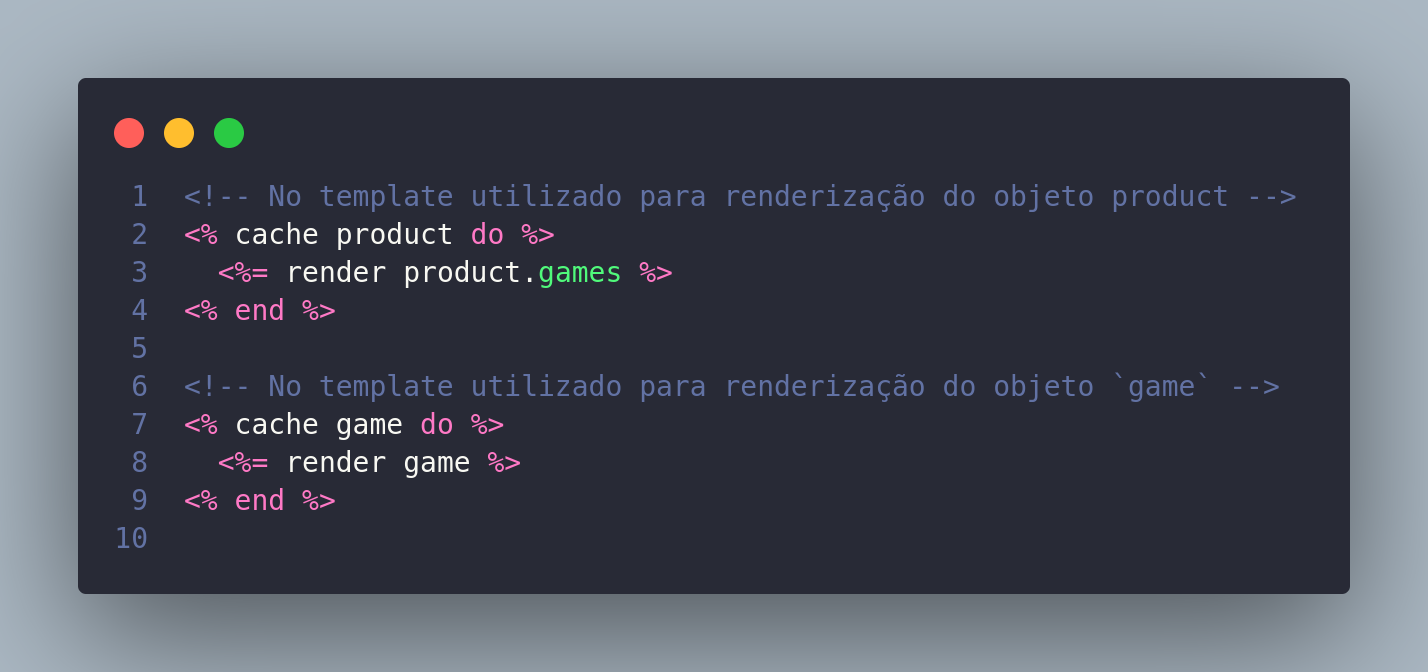
\includegraphics[width=0.7\textwidth]{figuras/russian_doll_template_example.png}
    \fonte{\cite{caching-with-rails-overview}}
    \label{fig:russian_doll_template_example}
\end{figure}


\begin{figure}
    \centering
    \caption{Inclusão da opção \textit{touch} na declaração de relacionamento entre \textit{models}}
    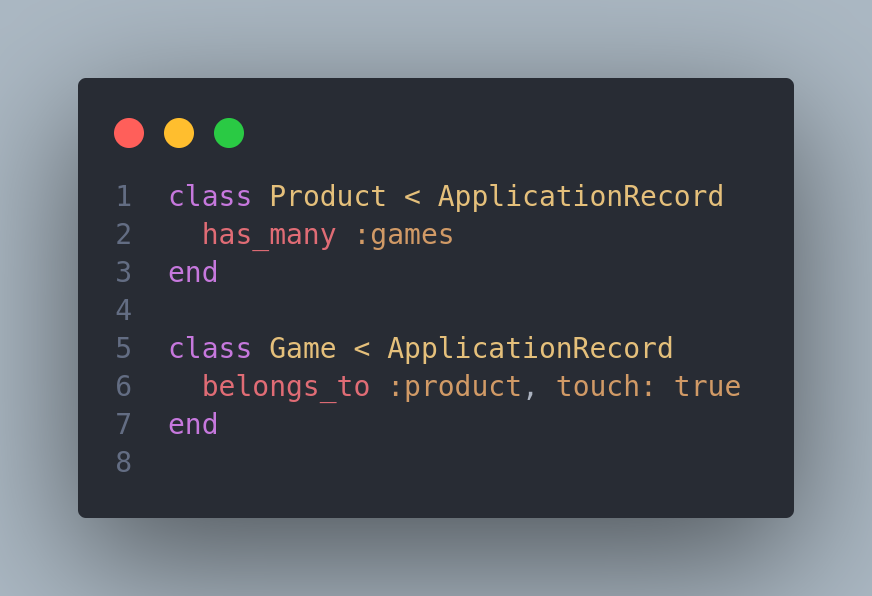
\includegraphics[width=0.7\textwidth]{figuras/russian_doll_touch_true.png}
    \fonte{\cite{caching-with-rails-overview}}
    \label{fig:russian_doll_touch_true}
\end{figure}

\subsection{Bases de dados para cache no Ruby on Rails}
\label{sec:bases_de_dados_para_cache_no_ruby_on_rails}

Como mencionado anteriormente, o \textit{Ruby on Rails} provê uma interface para comunicação com diversas tecnologias de armazenamento de \textit{cache}. Ele permite com que o programador especifique qual tecnologia deve ser utilizada na aplicação, e fornece uma interface que provê a fundação para interação com o sistema de \textit{cache}. Essa interface é o \textit{ActiveSupport::cache::Store}, que fornece métodos básicos para o programador: \textit{read}, \textit{write}, \textit{delete}, \textit{exist?}, e \textit{fetch}. Existem implementações dessa interface providas pelo \textit{Rails}, chamadas de \textit{Cache Store}, cujo propósito é operar com tecnologias de armazenamento conhecidas. Essas implementações são: o \textit{Memory Store}, o \textit{File Store}, o \textit{Mem \textit{cache} Store}, o \textit{Redis cache Store}, e o \textit{Null Store}; além de permitir o uso de \textit{Cache Stores} customizados.

\subsubsection{Memory Store}

O \textit{Memory Store} é uma tecnologia de armazenamento que utiliza a memória do próprio processo \textit{Ruby} em execução para guardar os registros. Esse \textit{cache store} possui as seguintes propriedades:

\begin{itemize}
    \item O tamanho do armazenamento é fixo, e deve ser especificado na configuração da aplicação;
    \item Sempre que faltar espaço para inserir novos registros, uma limpeza será realizada removendo os registros que não foram utilizados recentemente;
    \item No caso da aplicação estar rodando em múltiplos processos, um processo não terá acesso ao \textit{cache} do outro.
\end{itemize}

\subsubsection{File Store}

O \textit{File Store}, como o próprio nome sugere, utiliza o próprio sistema de arquivos para guardar os registros de \textit{cache}. Esse \textit{cache store} possui as seguintes propriedades:

\begin{itemize}
    \item O caminho do diretório utilizado para \textit{cache} é especificado na configuração da aplicação;
    \item No caso da aplicação estar rodando em múltiplos processos no mesmo \textit{host}, todos eles terão acesso ao mesmo \textit{cache}.
    \item O volume de dados utilizado pelo armazenamento de \textit{cache} cresce até que o disco se encontre cheio, sendo necessária a limpeza de registros antigos.
\end{itemize}

\subsubsection{Mem cache Store}

O \textit{Mem cache Store} é uma tecnologia de armazenamento de \textit{cache} baseada no \textit{memcached server} da \textit{Danga}. O \textit{Rails} utiliza a \textit{gem dalli} para operar com esse sistema de \textit{cache}, por padrão. Esse \textit{cache} \textit{store} possui a seguinte propriedade:

\begin{itemize}
    \item É possível utilizar um \textit{cluster} de servidores \textit{memcached}, porém, esses devem ser especificados na configuração da aplicação ou via variável de ambiente.
\end{itemize}

\subsubsection{Redis cache Store}

O \textit{Redis cache Store}, como o próprio nome sugere, é um \textit{cache store} que utiliza o \textit{Redis} como tecnologia de armazenamento de \textit{cache}. Esse \textit{cache store} possui as seguintes propriedades:

\begin{itemize}
    \item Dada a natureza do uso, é recomendado que se utilize um servidor \textit{Redis} dedicado para \textit{cache}.
    \item Servidores de \textit{cache Redis} permitem utilizar políticas de expiração de registros por: registro utilizado com menor frequência, ou registro que não é utilizado a mais tempo.
    \item O \textit{Redis cache Store} permite especificar parâmetros como: \textit{timeout} para conexão, \textit{timeout} para leitura, \textit{timeout} para escrita e tentativas de reconexão.
    \item O tempo gasto para criar ou reescrever um registro em \textit{cache} é pequeno, sendo as vezes mais vantajoso reescrever um registro do que esperar muito tempo para buscá-lo.
\end{itemize}